Complex systems require detailed architectural planning early on in the design process. The \abbreviationFull[Department of Defense]{DoD} attempted to manage the “Enterprise-level Architectures” and “Solution Architectures” throughout the department by publishing the \abbreviationFull[Department of Defense Architecture Framework]{DoDAF}. DoDAF defined an architecture as a “fundamental organization of a system embodied in its components, their relationships to each other and to its environment, and the principles governing its design and evolution over time \citep{DoDAF}.” This concept sounds reasonable, but system architects are not always available for every project that could benefit from a detailed architecture. Reference Architectures help alleviate that problem by consolidating subject matter expertise and previous relevant architectures into digestible models that system designers can benefit from when creating a Solution Architecture \citep{Cloutier2010}. The DoD saw the benefits of Reference Architectures and put out a Reference Architecture Description in 2010, describing them as “an authoritative source of information about a  specific subject area that guides and constrains the instantiations of multiple  architectures and solutions \citep{RADescription}," as shown in Figure \ref{fig:Ref Arc Purpose}.

\begin{figure}[!h]
    \centering
    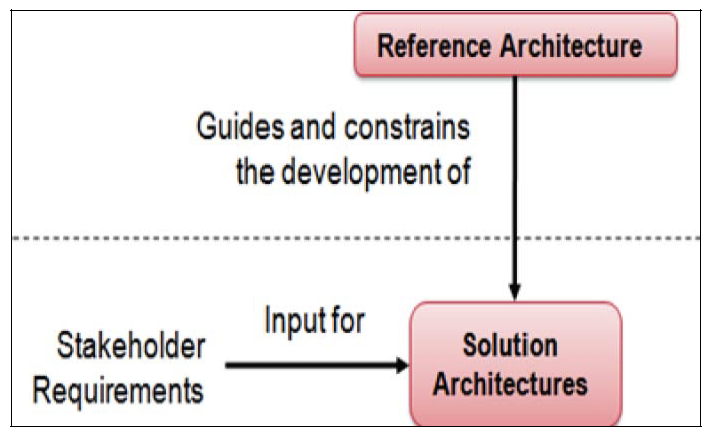
\includegraphics[width=3in]{Thesis/Literature_Review/Lit Review Figures/Ref Arc Purpose.png}
    \caption{Reference Architecture Purpose}
    \label{fig:Ref Arc Purpose}
\end{figure}

Cloutier \textcolor{red}{(introduce Cloutier and transition to this section better)} suggests 2 key principles for Reference Architectures.
\begin{enumerate}
\item{\textbf{Principle 1:} A Reference Architecture is an elaboration of company (enterprise) or consortium mission, vision, and strategy.   …facilitates a shared understanding about the current architecture and the vision on the future direction.}
\item{\textbf{Principle 2:} A Reference Architecture is based on concepts proven in practice. Preceding architectures can be mined for proven concepts.}
\end{enumerate}

Finally, Reference Architectures should have at least the following elements:
\begin{enumerate}
\item{\textbf{Strategic Purpose:} Goals, objectives, and a specific purpose or problem to be addressed}
\item{\textbf{Principles:} High-level foundational statements of rules, culture, and values that drive  technical positions and patterns}
\item{\textbf{Technical Positions:} Technical guidance and standards that must be followed by solution  architectures (maybe data vocabulary/ data model)}
\item{\textbf{Patterns (Templates):} Generalized representations (e.g., Viewpoints, Views, Diagrams, Products, Artifacts) showing relationships between elements specified in the Technical Position}
\item{\textbf{Vocabulary:} acronyms, terms, definitions}
\end{enumerate}

In summary, Reference Architectures can help systems engineers by providing a template, developed from years of experience, to aid in the systems engineering process. From the literature, it is clear that a Reference Architecture would be particularly useful for teams designing a CubeSat.

